



\part{Background}
\label{part:background}

%======================================================================
\chapter{Physics at the mesoscale}
\label{ch:swimming at the mesoscale}

\markright{Swimming at the mesoscale}
%======================================================================

\section{Low Renolds number regime}
\label{st:lowreynoldsnumber}

At the mesoscale, where objects such as bacteria and colloidal particles operate, the physical world is governed by a regime in which viscous forces dominate over inertial ones. This regime is characterized by a small Reynolds number (Re), a dimensionless quantity that compares inertial to viscous effects. Therefore, the force applied at that moment will describe the movement or displacement performed, not deppending on any past force, this is a characteristic of an overdamped system. In his seminal lecture, Life at Low Reynolds Number, Purcell highlighted the surprising and often counterintuitive behaviors that emerge in such environments \cite{purcell2014life}. For instance, time-reversible motion — common at macroscopic scales — is ineffective for propulsion at low Re, necessitating non-reciprocal strategies like flagellar rotation or body undulation. This leads to the scallop theorem, that states that an animal with such degrees of freedom — in a viscous regime — will not have a net displacement. 

This whole process can be described by the Navier-Stokes equation without the inertia terms, leaving us without any time deppending terms as shown in \ref{eq:Navier-Stokes}. 

\begin{equation}
  - \nabla p + \eta \nabla ^2 \vec{v} = 0
  \label{eq:Navier-Stokes}
\end{equation}

This has been a topic of interest for researchers that are constantly looking for ways of transportation in those environments for specific tasks. Unfortunately this is not the only challenge we face when moving at the microscale.

\section{Brownian Motion and Thermal Fluctuations}
\label{st:brownianmotion}

Even though this is a viscous regime, particles are not static. At small length scales, such as those of colloidal particles or bacteria, random thermal fluctuations become a dominant source of motion. This phenomenon, known as \textit{Brownian motion}, was first explained quantitatively by Albert Einstein in 1905. He demonstrated that the irregular paths observed in microscopic particles suspended in fluid result from collisions with the molecules of the surrounding medium~\cite{einstein1906theory}.

Einstein's work provided one of the first convincing arguments for the molecular nature of matter and led to a mathematical description of how these random movements accumulate over time. Specifically, he derived that the mean squared displacement (MSD) of a particle grows linearly with time:

\begin{equation}
  \langle x^2(t) \rangle = 2Dt\text{,}
  \label{eq:msd}
\end{equation}

where $D$ is the diffusion coefficient, a measure of how quickly particles spread out. Einstein further related this coefficient to measurable physical parameters through the expression:

\begin{equation}
  D = \frac{k_{B}T}{6\pi \eta R}\text{,}
  \label{eq:diffusioncoefficient}
\end{equation}

where $k_B$ is Boltzmann’s constant, $T$ the absolute temperature, $\eta$ the dynamic viscosity of the fluid, and $R$ the radius of the spherical particle. This relation — often referred to as the \textit{Einstein-Stokes equation} — is foundational in soft matter and colloidal physics.

In the systems considered in this thesis, Brownian motion plays a crucial role in the dynamics of passive colloids and must be accounted for even in the presence of external fields or active agents, such as bacteria.

\vspace{1em}

While Einstein’s formulation captures the long-term diffusive behavior of Brownian particles, it does not account for their instantaneous dynamics. To describe how particles move under both viscous damping and random thermal forces, we turn to a stochastic differential equation known as the \textit{Langevin equation}.

\subsection{Stochastic Representation}

The Langevin equation \cite{uhlenbeck1930theory} in one dimension, including inertial effects, damping, and thermal noise, can be written as:

\begin{equation}
  m\ddot{x} = F - \lambda \dot{x} + \eta(t)\text{,}
  \label{eq:newton}
\end{equation}

where $m$ is the particle mass, $\lambda$ is the damping coefficient, and $\eta(t)$ is a stochastic force representing thermal noise. For simplicity, we write the velocity as $v = \dot{x}$, leading to:

\begin{equation}
  m\frac{dv}{dt} = F - \lambda v + \eta(t)\text{.}
  \label{eq:newtonv}
\end{equation}

Discretizing time with a small step $dt$, we apply the definition of a derivative:

\begin{equation}
  m \frac{v(t + dt) - v(t)}{dt} = F - \lambda v(t) + \eta(t)\text{.}
  \label{eq:newtonderivative}
\end{equation}

The thermal noise term $\eta(t)$ is modeled as a Gaussian white noise process:

\begin{equation}
  \eta(t)\, dt = g\, dW\text{,}
  \label{eq:eta}
\end{equation}

where $dW$ is a Wiener process (increment of Brownian motion) such that:

\begin{equation}
  \langle dW \rangle = 0\,, \quad \langle dW^2 \rangle = dt\text{.}
  \label{eq:meanvariance}
\end{equation}

Solving for $v(t + dt)$ gives:

\begin{equation}
  v(t + dt) = v(t) + \frac{dt}{m}(F - \lambda v(t)) + g\, dW\text{.}
  \label{eq:velocityplusone}
\end{equation}

Now, assuming no deterministic force ($F = 0$) — as is the case for free passive particles:

\begin{equation}
  v(t + dt) = v(t) - \frac{\lambda dt}{m} v(t) + g\, dW\text{.}
  \label{eq:noforce}
\end{equation}

Taking the expectation value (mean) of both sides:

\begin{equation}
  \langle v(t + dt) \rangle = \langle v(t) \rangle - \frac{\lambda dt}{m} \langle v(t) \rangle + g \langle dW \rangle\text{.}
  \label{eq:mean}
\end{equation}

Since $\langle dW \rangle = 0$, the last term vanishes:

\begin{equation}
  \langle v(t + dt) \rangle = \langle v(t) \rangle \left( 1 - \frac{\lambda dt}{m} \right)\text{.}
\end{equation}

In the limit of small $dt$, this leads to the differential equation:

\begin{equation}
  \frac{d}{dt} \langle v(t) \rangle = - \frac{\lambda}{m} \langle v(t) \rangle\text{,}
  \label{eq:derivative}
\end{equation}

whose solution is:

\begin{equation}
  \langle v(t) \rangle = \langle v(0) \rangle\, e^{-\lambda t / m}\text{.}
\end{equation}

This result shows that the average velocity of a particle in a viscous fluid decays exponentially due to damping. The characteristic timescale $\tau = m/\lambda$ describes how quickly the particle forgets its initial velocity, after which the motion becomes diffusive.

%%%%

\subsection{Velocity Statistics and Energy Equipartition}

To compute the variance of the velocity, we start again from the Langevin equation in discretized form, without external forces:

\begin{equation}
  v(t + dt) = v(t) - \frac{\lambda}{m} v(t) dt + \frac{g}{m} dW \text{.}
\end{equation}

Squaring both sides:

\begin{align}
  v(t + dt)^2 &= \left[ v(t) - \frac{\lambda}{m} v(t) dt + \frac{g}{m} dW \right]^2 \text{,}\\
              &= v(t)^2 + \left( \frac{\lambda}{m} \right)^2 v(t)^2 dt^2 + \left( \frac{g}{m} \right)^2 dW^2 \nonumber \\
              &\quad - 2 \frac{\lambda}{m} v(t)^2 dt + 2 \frac{g}{m} v(t) dW - 2 \frac{\lambda g}{m^2} v(t) dW \text{.}
\end{align}

Now we take the expectation value:

\begin{align}
  \langle v(t + dt)^2 \rangle &= \langle v(t)^2 \rangle + \left( \frac{\lambda}{m} \right)^2 \langle v(t)^2 \rangle dt^2 + \left( \frac{g}{m} \right)^2 \langle dW^2 \rangle \nonumber \\
                              &\quad - 2 \frac{\lambda}{m} \langle v(t)^2 \rangle dt + 2 \frac{g}{m} \langle v(t) \rangle \langle dW \rangle - 2 \frac{\lambda g}{m^2} \langle v(t) \rangle \langle dW \rangle \text{.}
\end{align}

Using the properties of the Wiener process:

\[
  \langle dW \rangle = 0, \quad \langle dW^2 \rangle = dt \text{.}
\]

And neglecting second-order small terms (\( dt^2 \)), we obtain:

\begin{equation}
  \langle v(t + dt)^2 \rangle = \langle v(t)^2 \rangle + \frac{g^2}{m^2} dt - 2 \frac{\lambda}{m} \langle v(t)^2 \rangle dt \text{.}
\end{equation}

Taking the continuous limit:

\begin{equation}
  \frac{d}{dt} \langle v(t)^2 \rangle = -2 \frac{\lambda}{m} \langle v(t)^2 \rangle + \frac{g^2}{m^2} \text{.}
\end{equation}

This is a linear first-order ODE. Solving it with variation of constants yields:

\begin{equation}
  \langle v(t)^2 \rangle = \frac{g^2}{2 \lambda m} + D e^{-2 \lambda t / m} \text{.}
\end{equation}

As \( t \to \infty \), the exponential term vanishes and we get the stationary value:

\begin{equation}
  \langle v(\infty)^2 \rangle = \frac{g^2}{2 \lambda m} \text{.}
\end{equation}

From the equipartition theorem, we know that the average kinetic energy is:

\[
  \frac{1}{2} m \langle v^2 \rangle = \frac{1}{2} k_B T \text{.}
\]

Therefore:

\begin{equation}
  \langle v^2 \rangle = \frac{k_B T}{m} \text{.}
\end{equation}

Matching this to our stochastic result:

\begin{equation}
  \frac{k_B T}{m} = \frac{g^2}{2 \lambda m} \quad \Rightarrow \quad g^2 = 2 \lambda k_B T, \quad g = \sqrt{2 \lambda k_B T} \text{.}
\end{equation}

This defines the noise amplitude in terms of temperature, viscosity, and Boltzmann’s constant.

\subsection{Overdamped Dynamics and Diffussion}

In the overdamped limit, inertia is negligible, so the Langevin equation becomes:

\begin{equation}
  0 = F - \lambda \frac{dx}{dt} + \eta(t) \text{.}
\end{equation}

Solving for the velocity:

\begin{equation}
  \frac{dx}{dt} = \frac{1}{\lambda} (F + \eta(t)) \text{.}
\end{equation}

For free diffusion (\( F = 0 \)):

\begin{equation}
  \frac{dx}{dt} = \frac{1}{\lambda} \eta(t) \text{.}
\end{equation}

Using stochastic calculus with \( \eta(t) dt = g dW \), we write:

\begin{equation}
  x(t + dt) = x(t) + \frac{g}{\lambda} dW \text{.}
\end{equation}

\paragraph{Mean Position}

Taking the expectation:

\begin{equation}
  \langle x(t + dt) \rangle = \langle x(t) \rangle + \frac{g}{\lambda} \langle dW \rangle = \langle x(t) \rangle \text{.}
\end{equation}

So the mean position remains constant in free diffusion.

\paragraph{Mean Square Displacement (MSD)}

Squaring the position update:

\begin{equation}
  x(t + dt)^2 = x(t)^2 + 2 \frac{g}{\lambda} x(t) dW + \left( \frac{g}{\lambda} \right)^2 dW^2 \text{.}
\end{equation}

Taking the expectation:

\begin{align}
  \langle x(t + dt)^2 \rangle &= \langle x(t)^2 \rangle + 2 \frac{g}{\lambda} \langle x(t) \rangle \langle dW \rangle + \frac{g^2}{\lambda^2} \langle dW^2 \rangle \text{,}\\
  &= \langle x(t)^2 \rangle + \frac{g^2}{\lambda^2} dt \text{.}
\end{align}

In differential form:

\begin{equation}
  \frac{d}{dt} \langle x(t)^2 \rangle = \frac{g^2}{\lambda^2} \text{.}
\end{equation}

Using \( g^2 = 2 \lambda k_B T \), we substitute:

\begin{equation}
  \frac{d}{dt} \langle x(t)^2 \rangle = \frac{2 k_B T}{\lambda} \text{.}
\end{equation}

Integrating gives the mean squared displacement (MSD):

\begin{equation}
  \langle x(t)^2 \rangle = \frac{2 k_B T}{\lambda} t \text{.}
\end{equation}

This is the classical diffusion result, where the diffusion coefficient is \( D = \frac{k_B T}{\lambda} \), consistent with Einstein's expression.



%%%%
%This raises a fundamental question: Can these fluctuations be harnessed to perform useful work? This idea lies at the heart of thought experiments such as the Feynman ratchet, which challenge our understanding of thermodynamics at microscopic scales.


\begin{figure}[H]
  \begin{center}
    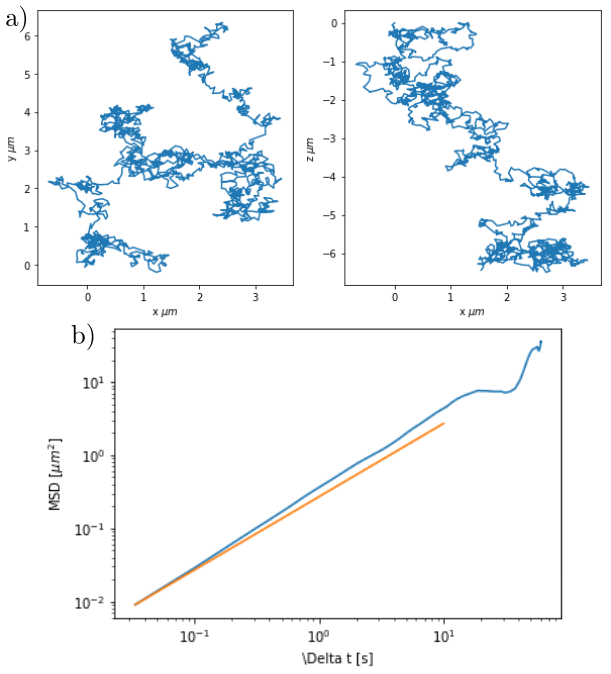
\includegraphics[width=0.8\textwidth]{figures/passivebrowniantrajectorymsd.png}
  \end{center}
  \caption[Example of brownian motion]{A colloidal particle undergoes random, thermally induced displacements in a fluid medium. \textbf{Panel a)} shows the trajectory of the particle. \textbf{ Panel b)} shows the corresponding mean squared displacement (MSD) as a function of time, illustrating the linear relationship predicted by Einstein for diffusive behavior (orange) and the one obtained through a numerical simulation (blue).}\label{fig:passivebrowniantrajectory}
\end{figure}

\chapter{Ratchets and Rectification Mechanisms}
\label{ch:ratchetsandrectificationmechanisms}

\section{The Feynman-Smoluchowski ratchet}

The inherent randomness of Brownian motion naturally leads to the question: can this disorder be transformed into order? In other words, can the random thermal motion of particles be used to produce directed movement or extract work? This question sits at the core of statistical mechanics and was famously explored by Richard Feynman in his lectures on physics, through a thought experiment known as the Feynman ratchet and pawl \cite{feynman1963feynman}.

The Feynman ratchet consists of a set of vanes connected to a ratchet wheel, immersed in a fluid (Fig. \ref{fig:feynmanratchet}). The idea is: random collisions from the surrounding molecules could push the vanes, but the pawl only allows rotation in one direction. At first glance, this asymmetric mechanism seems capable of converting random thermal motion into unidirectional rotation, apparently violating the second law of thermodynamics.

\begin{figure}
  \begin{center}
    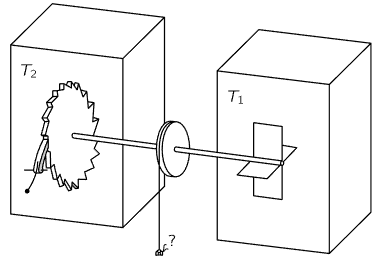
\includegraphics[width=0.65\textwidth]{figures/feynmanratchet.png}
  \end{center}
  \caption[Feynman ratchet]{Visual representation of the Feynman ratchet. Obtained from \cite{feynman1963feynman}}\label{fig:feynmanratchet}
\end{figure}


However, Feynman's analysis showed that when both the ratchet and the pawl are in thermal equilibrium with the same heat bath, the system cannot produce net work. The pawl itself undergoes thermal fluctuations and can occasionally lift off, allowing the ratchet to move backward. Over time, the forward and backward movements average out, and no net rotation occurs. This result reinforces the principle that thermal fluctuations alone cannot be rectified to perform work without a temperature gradient or an external energy input.

\begin{table}[ht]
\centering
\renewcommand{\arraystretch}{1.4}
\caption[Summary of operation of ratchet and pawl.]{Summary of operation of ratchet and pawl. Obtained from \cite{feynman1963feynman}}
\label{tab:ratchet_pawl}
\begin{tabular}{>{\itshape}l l l}
\toprule
\textbf{Forward:} & Needs energy & $\epsilon + L \theta$ from vane. \quad $\therefore$ Rate = $\dfrac{1}{\tau} e^{-(L\theta + \epsilon)/kT_1}$ \\
                  & Takes from vane & $L\theta + \epsilon$ \\
                  & Does work & $L\theta$ \\
                  & Gives to ratchet & $\epsilon$ \\
\midrule
\textbf{Backward:} & Needs energy & $\epsilon$ for pawl. \quad $\therefore$ Rate = $\dfrac{1}{\tau} e^{-\epsilon/kT_2}$ \\
                   & Takes from ratchet & $\epsilon$ \\
                   & Releases work & $L\theta$ \\
                   & Gives to vane & $L\theta + \epsilon$ \\
\bottomrule
\end{tabular}

\vspace{1em}
If system is reversible, rates are equal, hence 
\[
\frac{\epsilon + L\theta}{T_1} = \frac{\epsilon}{T_2}.
\]
\[
\frac{\text{Heat to ratchet}}{\text{Heat from vane}} = \frac{\epsilon}{L\theta + \epsilon}.
\quad \text{Hence} \quad \frac{Q_2}{Q_1} = \frac{T_2}{T_1}.
\]
\end{table}

Despite this limitation, the Feynman ratchet introduced a powerful concept: asymmetry combined with non-equilibrium conditions can, in principle, produce directed motion. This idea is foundational in the study of Brownian motors, biomolecular machines, and active matter systems, including the systems explored in this thesis. In such systems, energy is continuously supplied, whether through bacterial metabolism or magnetic field modulation, creating the necessary non-equilibrium environment that allows motion rectification to occur.

The failure of the Feynman ratchet in thermal equilibrium is intimately connected to another famous thought experiment: Maxwell's demon. Both systems attempt to extract work from thermal fluctuations through selective processes—the ratchet through mechanical asymmetry, and the demon through information gathering.

Maxwell's demon, proposed in 1867, imagines a microscopic being that can sort fast and slow molecules between two chambers, creating a temperature difference without apparent work. Similarly, the pawl in Feynman's ratchet acts as a mechanical "demon," attempting to select only forward fluctuations while blocking backward motion. However, both fail for the same fundamental reason: the cost of selection itself \cite{maxwell1871theory, maxwell1867letter}.

Brillouin (1951) and later Landauer (1961) showed that Maxwell's demon must expend energy to measure molecular velocities and erase information, with the minimum energy cost being $kT\ln{2}$ per bit erased. In the Feynman ratchet, the pawl must "decide" whether to allow motion, and this decision-making process—manifested as thermal fluctuations of the pawl itself—has an entropic cost that exactly cancels any work extracted \cite{brillouin1951maxwell, landauer1961irreversibility}.

This connection reveals a deep principle: rectification requires either an information gradient (knowledge about the system) or an energy gradient (non-equilibrium conditions). As Parrondo and Español (1996) demonstrated, the Feynman ratchet can be viewed as an information engine where the pawl performs measurements on the ratchet's position. When the pawl and ratchet are at the same temperature, the information gained equals the entropy produced, yielding no net work \cite{parrondo1996criticism}.


\section{Brownian ratchets and tilted potentials}

While Feynman's ratchet fails due to thermal equilibrium, rectified motion becomes possible when detailed balance is broken through external driving. Magnasco (1993) demonstrated this principle through the "rocking ratchet" mechanism \cite{magnasco1993forced}. In his model, a Brownian particle moves in an asymmetric periodic potential—essentially a sawtooth-shaped energy landscape with gentle slopes in one direction and steep walls in the other.
The crucial innovation was applying an oscillating force $F(t) = A\cos(\omega t)$ that rocks the potential back and forth. Although this force has zero time average—pushing equally left and right—the combination with the spatial asymmetry produces net directional motion. When the force tilts the potential forward, particles easily climb the gentle slopes and can overcome barriers. When tilted backward, particles encounter steep walls and remain trapped. This asymmetric response to symmetric driving breaks the forward-backward symmetry of thermal diffusion.

This mechanism differs fundamentally from Feynman's original ratchet: rather than attempting to rectify equilibrium fluctuations (which violates the second law), the rocking ratchet continuously injects energy through the oscillating force. The time-dependent driving maintains the system far from equilibrium, enabling the spatial asymmetry to generate directed transport. This principle—that asymmetry plus non-equilibrium driving yields rectification—underlies numerous biological processes and provides the theoretical foundation for the magnetically-driven ratchets explored in this thesis.

\section{Geometric ratchets}

Unlike energy ratchets that rely on asymmetric potentials, geometric ratchets achieve rectification through spatial asymmetry of boundaries or obstacles, particularly relevant for self-propelled particles

\chapter{Active Matter Systems}
\label{ch:activeandpassivemattersystems}

\section{Fundamentals of Active Matter}

Active matter refers to systems composed of self-driven units that continuously consume energy from their environment to propel themselves \cite{marchetti2013hydrodynamics, ramaswamy2010mechanics}. It is important to note it doesn't matter if the particles are artificial or oganic. The difference of active particles from passive ones, is that passive have mere diffusion motion, whereas active follows these stochastic differential equations accordnig to \cite{volpe2014simulation}:
\begin{align}
  \frac{d}{dt}x(t) &= v\cos{\varphi(t)} + \sqrt{2D_T}W_x,\\
  \frac{d}{dt}y(t) &= v\sin{\varphi(t)} + \sqrt{2D_T}W_y,\\
  \label{eq:activestochasticequation}
\end{align}

where $W_x$, and $W_y$ represent their corresponding Wiener process. As stated before, if 

\begin{equation}
  \lim_{v \to 0}  v\cos{\varphi(t)} + \sqrt{2D_T}W_x,
  \label{eq:limitofvelocity}
\end{equation}

then the motion is merely diffusive and the particle is characterized as brownian particle. Figure \ref{fig:msddifferentvelocities} helps visualize how  the motion varies according to their velocity. When the velocity is zero, the linear behavior of the MSD represents a diffusive behavior, whereas when it is different it is considered to be ballistic. 

\begin{figure}
  \begin{center}
    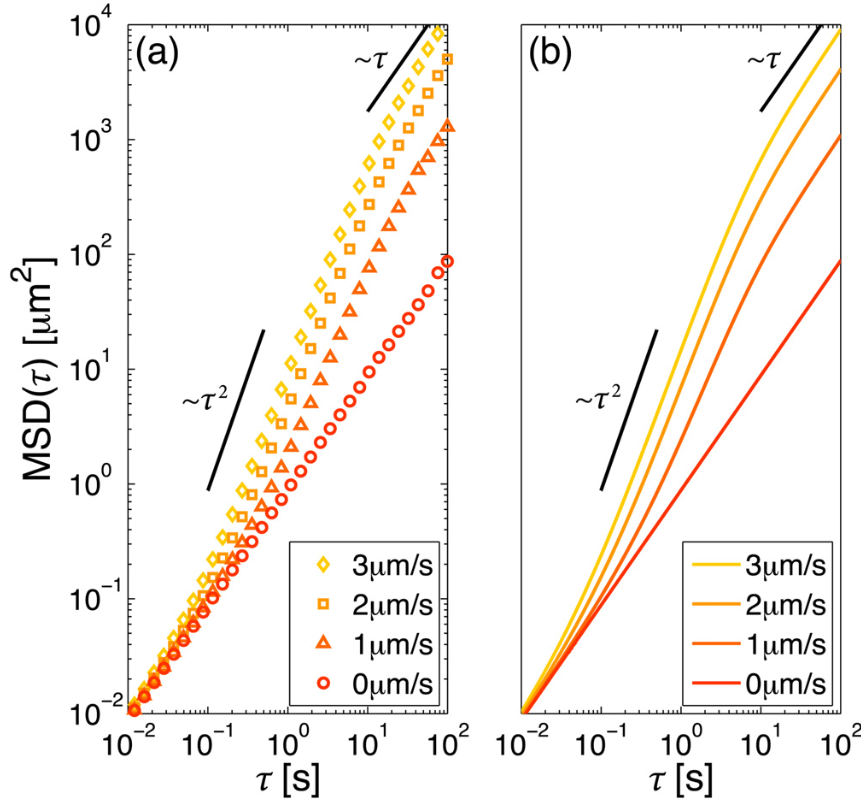
\includegraphics[width=0.55\textwidth]{figures/msddifferentvelocities.png}
  \end{center}
  \caption[MSD for passive and active brownian particles]{MSD for brownian particles with different velocites. \textbf{Panel a)} shows the result from simulations. \textbf{Panel b)} shows the theoretical calculation. Obtained from \cite{volpe2014simulation}}\label{fig:msddifferentvelocities}
\end{figure}


The foundational work by Howse et al. (2007) established the experimental basis for active Brownian particle dynamics by studying self-motile colloidal particles that use chemical reactions catalyzed on their surface to achieve autonomous propulsion. They demonstrated that at short times, these particles exhibit substantial directed motion with velocity dependent on fuel concentration, while at longer times, the motion transitions to a random walk with enhanced diffusion coefficients. This work provided the first comprehensive experimental validation of the theoretical active Brownian particle model and established the standard mathematical framework for describing such systems through coupled stochastic differential equations \cite{howse2007self}.


As discussed in section \ref{st:lowreynoldsnumber}, organisms or objects must break symmetry in specific ways to achieve net movement when swimming in environments dominated by viscous forces. Nature has evolved elegant solutions to this challenge through various biological mechanisms. A prime example is E. coli, which employs helical flagella that can rotate both clockwise and counterclockwise, generating two distinct types of motion that researchers have termed "run" and "tumble." The bacterium's response to random fluctuations also depends on the medium's viscosity \cite{kumar2010physics}.

The dynamics of active particles exhibit fascinating collective behaviors that have drawn inspiration from biological systems. A computational study by Reynolds (1987) used simulations to model flocking behavior in birds, treating each individual as an autonomous agent whose trajectory is influenced by its local environment and neighboring individuals \cite{reynolds1987flocks}. Reynolds introduced three fundamental rules governing flocking behavior: separation (collision avoidance), alignment (velocity matching with neighbors), and cohesion (attraction toward the average position of neighbors). This work established the foundation for understanding how simple local interactions can give rise to complex collective motion patterns. The principles identified by Reynolds have since been adapted and extended to describe the collective dynamics of active Brownian particles, where similar emergent behaviors such as clustering, swarming, and directed group motion arise from the interplay between self-propulsion and inter-particle interactions.

\section{Interaction with non-homogeneous environments}

All this properties considered an ideal environment, where no obstacles are present. Active particles in real environments encounter surfaces, confinement, and flow fields that dramatically alter their behavior. A striking example is the work by Hill et al. (2007), who demonstrated that E. coli swimming near surfaces in shear flow exhibit sophisticated rheotaxis - the ability to sense flow gradients and actively swim upstream through hydrodynamic surface interactions \cite{hill2007hydrodynamic}. 

\section{Active Ratchets: State of the Art}


\chapter{Magnetically Driven Colloidal Systems}
\label{magneticallydrivencolloidalsystems}

\section{Magnetic Colloids under static fields}

\section{Dynamic Magnetic Actuation}

Active matter requires a continuous source of energy to avoid falling under the category of Brownian particles. However, for complex challenges—such as transportation—these systems can tend to be inefficient due to their energy depletion.

Fortunately, Ostinato et al. (2024)
Dimer formation, exchange dynamics

Emergent currents withouth self-propulsion

In the study of motion at small scales, materials are often categorized as either active or passive. This distinction is based on whether the constituents are capable of autonomously converting energy into motion.


This thesis focuses on such externally driven passive systems, particularly on paramagnetic colloids subjected to dynamic magnetic fields. These systems provide a controlled platform to study non-equilibrium transport and rectified motion, drawing inspiration from active matter while remaining fundamentally passive in nature.

\newpage
